% Author: PokMan Ho
% Script: apdx.tex
% Desc: MRes thesis appendix section
% Input: none
% Output: none
% Arguments: 0
% Date: Jun 2020

\documentclass[../thesis.tex]{subfiles} %% use packages & commands as this main file

\begin{document}
\section{Appendix}
\beginSupp
%this is an appendix

\subsection{Features comparison between models}
\begin{table}[H]
\begin{tiny}
    \centering
    \caption[Model features comparison]{Table of features comparison (18 features) between model in this project with aquatic slab models (23 models) and two terrestrial nutrient cycle models}
    \csvautotabular[]{media/modComp1.csv}\\
    \vspace{.5cm}
    \csvautotabular[]{media/modComp2.csv}\\
    \vspace{.5cm}
    \csvautotabular[]{media/modComp3.csv}
    \label{modComp}
\end{tiny}
\end{table}

\subsection{Temperature-standardisation}
The procedure included two parts.  Parameter values collected from literature were temperature-tagged.  For parameters with very limited data points, majority of the data were collected under \temp.  Hence this study chose 23\textsuperscript{o}C as the standard reference to investigate with the proposed model.

Growth rate data was obtained from ``BioTrait" database\autocite{della2013thermal}.  Six filters were applied to extract published aquatic microbial \phy\ $P$ or \bac\ $B$ species entries which were identified to species level.  The matched data set was further filtered to eliminate entries reported no growth because these records could not reflect the temperature effect using the Arrhenius Equation.

\begin{equation}
    A = A_0e^{-\dfrac{E_a}{k(T_C+273.15)}}
    \label{arrEq}
\end{equation}

which $A$ is rate standardised in data and $A_0$ is the standardisation constant with the same unit, $E_a$ is the activation energy with unit eV, $k$ is Boltzmann constant from Scipy (v1.4.1) package under unit eV/K and $T_C$ is the temperature of the organism measured from the data with unit (\textsuperscript{o}C).

Activation energies for phytoplanktons and \bac\ are 0.32eV and 0.66eV respectively\autocite{regaudie2012temperature}.  Standardised rate unit in data was initially ``sec\textsuperscript{-1}" and the unit was re-standardised to ``\dayU" for this study (Fig.\ref{f:A0}).

\begin{figure}[H]
    \centering
    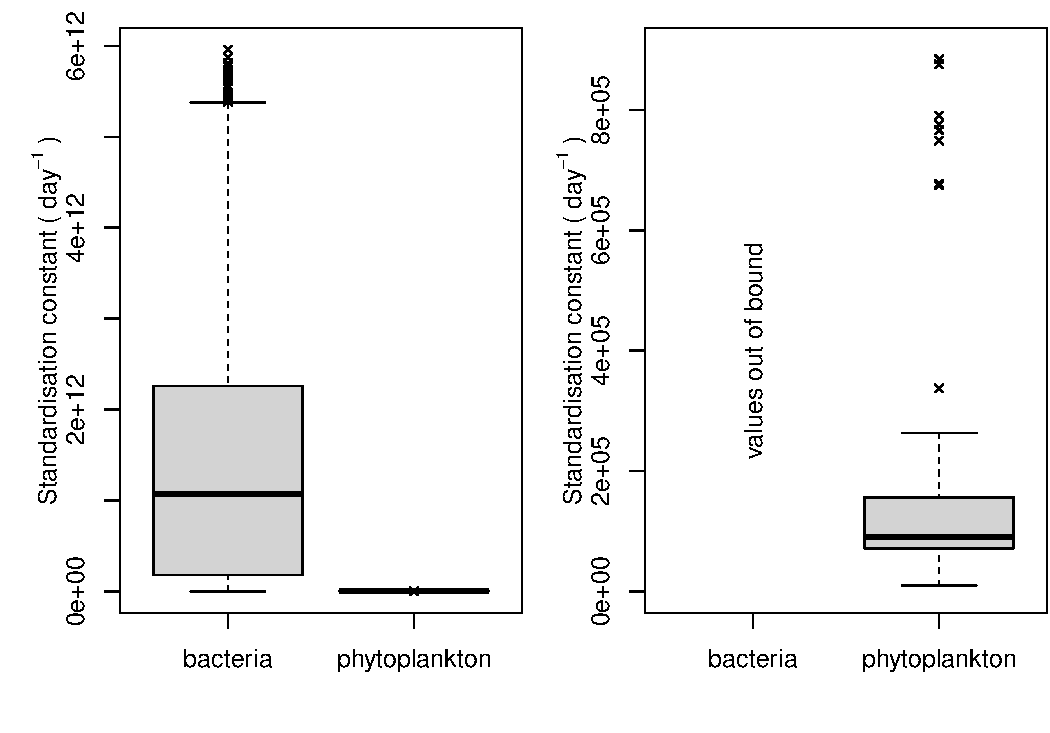
\includegraphics[width=\linewidth]{../result/stdCst.pdf}
    \caption[Boxplot of standardised $A_0$]{Boxplots of $A_0$ for \phy\ and \bac\ with unit ``\dayU"}
    \label{f:A0}
\end{figure}

Temperature-standardised growth rates were calculated by time-standardised and respective activation energies mentioned above.  The resultant data hence was in the unit of \dayU under 23\textsuperscript{o}C.

\subsection{\Phy\ growth rates data wrangling}
Percentage range of the temperature-standardised data was calculated by the deviation of rate extremes from the mean.  This range was also considered one of the candidates for rate parameters which did not have sufficient data (min data entries of 5) to construct their percentage ranges.

The parameter range was hence calculated by mean of the standardised \phy\ growth rates $\pm$ percentage range of its own.

\subsection{\Bac\ clearance rates data wrangling}
Temperature-time-standardised growth rate data from ``BioTrait" were not applicable directly due to the disagreement of units.  Clearance rate for microbes were also technically unfeasible to measure.  Yet these two quantities were related by the following linear relationship

\begin{equation}
    \text{[clearance]} \times \text{[resource density]} = \text{[growth]}
    \label{eq:gB}
\end{equation}

Due to the lack of data for resource density in literature collected by ``BioTrait" database \autocite{della2013thermal}, the only approach was using an arbitrary density (10 was used in this study) to resolve the unit issue.  The process was based on prior knowledge on cell size scaling of metabolism, so that the resultant ranges of growth rate is comparable between $P$ and $B$.

With data modifiable, percentage ranges of $\gB$ were calculated and parameter ranges were deduced using the same method mentioned above.  Its percentage range was also considered as a candidate for other similar parameters without sufficient data to construct a percentage range for its own.

\subsection{Parameter ranges for intraspecific interference of \phy\ and death rate of \bac}
Three and one data point(s) were available from reachable literature for $\aP$ \autocite{de2007biofixation} and $\mB$ \autocite{cochran1988estimation} respectively.  We chose the widest percentage range from available candidates in the same category for these rate parameters.  Percentage range of $\gP$ was hence selected as their reference range indicator in this study.  Their parameter ranges were calculated using the same approach explained in previous section.

For $\aP$ data collected from \autocite{de2007biofixation}, they were in 30\textsuperscript{o}C.  Although there was a temperature mismatch, they were still used because of no available data.  Hence it was assumed that the resultant parameter range could cover possible values in \temp.

\subsection{Non-respired carbon fraction for \phy\ data wrangling}
Data was available in the form of linear equations in \autocite{j1989respiration}.  These equations from literature was temperature-tagged with y-axis as respiration rate and x-axis as growth rate.  Hence only the equations within the considered temperature ranges were accepted.  Among the six equations matched , intercepts and slope values were collected.

Using the growth rates for \phy\ at 23\textsuperscript{o}C calculated, the non-respired fraction of carbon ($n(R')$) was deduced as

\begin{equation}
    n(R') = 1-n(R) = 1-\dfrac{[\text{intercept}]+[\text{slope}]\cdot\gP}{\gP}
    \label{ePReqn}
\end{equation}

Due to lack of matches between growth rate data and species available for these linear equations, the pool of parameter values were calculated by pairing every available growth rate with every available intercept-slope couple.  Percentage range was calculated and was considered as a candidate of reference range in the ``fraction" category.

Parameter range of $\ePR$ was calculated using the method described above but the maximum value was capped at 1 because in the proposed model it was assumed that P cannot absorb carbon from the C pool.

\subsection{Biomass assimilated carbon fraction for \phy\ data wrangling}
Two papers were containing values with temperature matches \autocite{j1989respiration,samejima1958heterotrophic}.  Due to the assumption of ``no absorption of organic carbon from $C$ pool by $P$", these fractions were capped at 1.  Percentage range for this wrangled data pool was calculated and considered as a reference candidate for the ``fraction" category.

Parameter range of $\eP$ was calculated with the above method with maximum capped at 1.

\subsection{Non-respired carbon fraction for bacterial decomposer parameter range calculation}
$\eBR$ was calculated from Fig.1b and glucose recovery rate values of \autocite{cochran1988estimation}.  This paper was also the only publication with values associated with its respected parameter.  In the figure a net 100mg of carbon originated from straw material was recovered per gram of straw at around 24-28 days (from day 0).  At that period, the recovery rate of carbon released by respiration originated from external glucose was 80\%.  Since in the environment carbon source was either external glucose or straw, the respired carbon fraction is $\dfrac{100\cdot10^{-3}}{28\cdot(1-0.8)}$ and the non-respired carbon fraction is (1-[respired fraction]).

The calculated value was treated as the parameter mean and the percentage range of $\ePR$ was selected as the reference range for deduction of possible parameter range for $\eBR$

\subsection{Biomass assimilated carbon fraction for bacterial parameter range calculation}
The only data was embedded in \autocite{cochran1988estimation} and was treated as the mean of its parameter range.  Percentage range of $\ePR$ was selected as its reference range to deduce the range values.

\subsection{Log yield flux comparisons between \phy-only and \pbs s (Fig.\ref{f:bacEffect} cont)}
\begin{figure}[H]
    \centering
    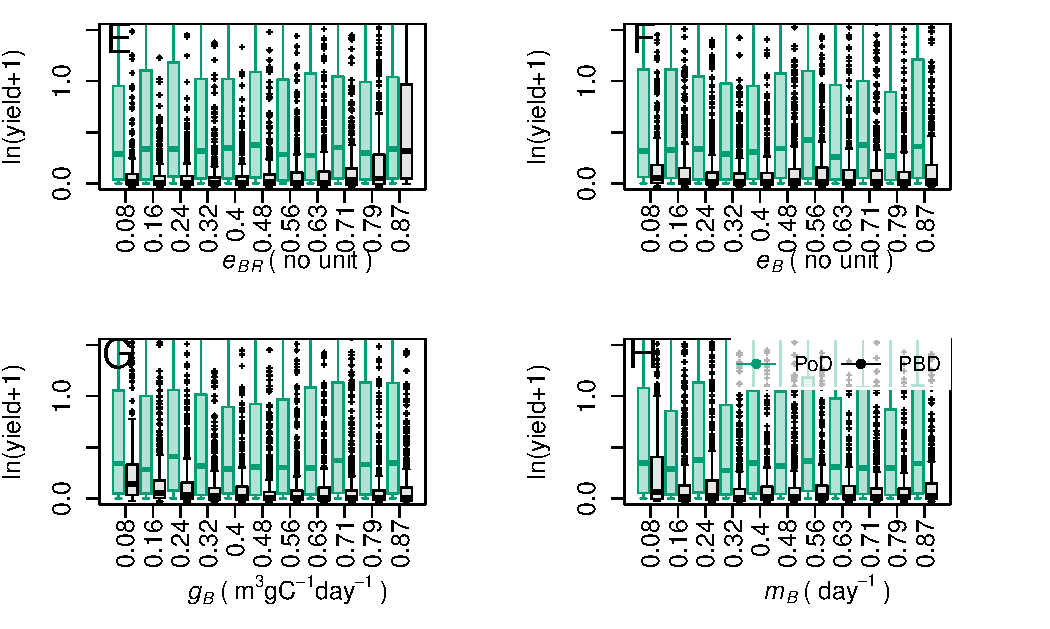
\includegraphics[width=.95\linewidth]{result/bacEff2.pdf}
    \caption[Log yield flux comparisons between \phy-only and \pbs s on \bac\ parameters]{Log yield flux comparisons between \phy-only and \pbs s on \bac\ parameters along respective parameter ranges under a standardised temperature range of \temp.  This is the second part of Fig.\ref{f:bacEffect}.  Full description of variables were in Table \ref{t:ranges}.  Each group in each plot has an LHS sample size of 5500.  Pairwise Wilcox test shows significance (p $\ll$ 0.01) between the systems.  Note that only a few scenarios of \pbs s are positives, which symbolise small feasibility.  Also note that ranges of both groups are similar, symbolising comparable yield values are possible for \pbs s when biologically compatible candidates are selected.}
    \label{f:bacEffect2}
\end{figure}

\subsection{Log yield flux comparisons between \pbs s}
\begin{figure}[H]
    \centering
    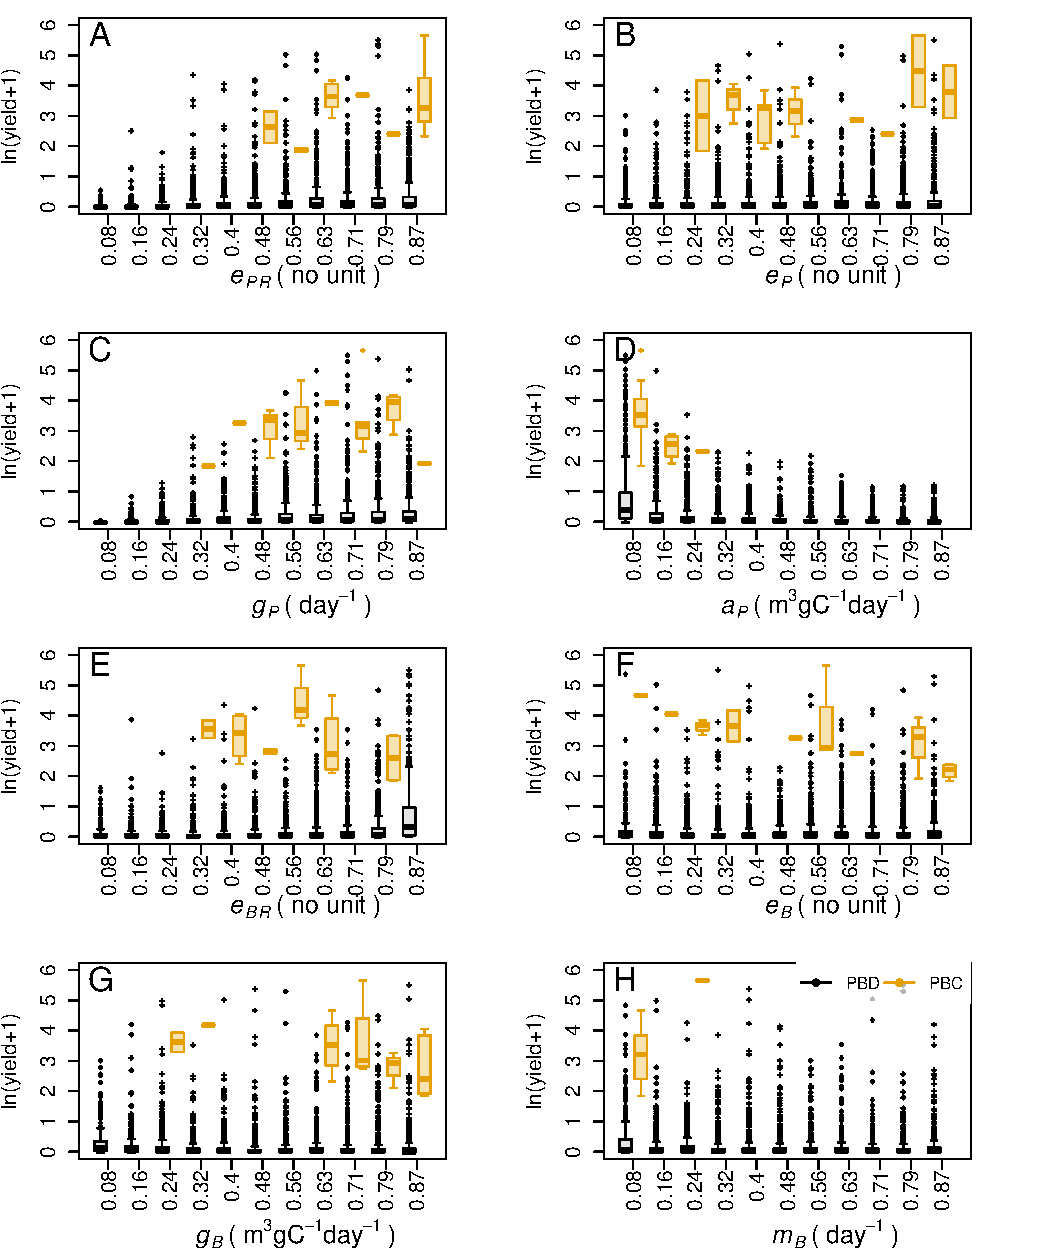
\includegraphics[width=.95\linewidth]{result/harvB.pdf}
    \caption[Log yield flux comparisons between \pbs s]{Log yield flux comparisons between \pbs s along respective parameter ranges under a standardised temperature range of \temp.  For each independent variable value, the box on its left represented \PBN\ while the one on the right represented \PBH.  Full description of variables were in Table \ref{t:ranges}.  Each group in each plot had an LHS sample size of 5500.  Pairwise Wilcox test showed significance (p $\ll$ 0.01) between the systems.  Note that only a few scenarios of \pbs s were positives, which symbolised small feasibility.  Also note that the highest value of \PBH\ was higher than that of \PBN\ systems, indicating the best scenario of continuous harvest systems yielded higher than that of \PBN.  Yet \PBN\ systems had more feasible scenarios (47.0\%) than \PBH\ ones (0.3\%).}
    \label{f:harvPB}
\end{figure}

\subsection{Log yield flux comparisons between \phy-only systems}
\begin{figure}[H]
    \centering
    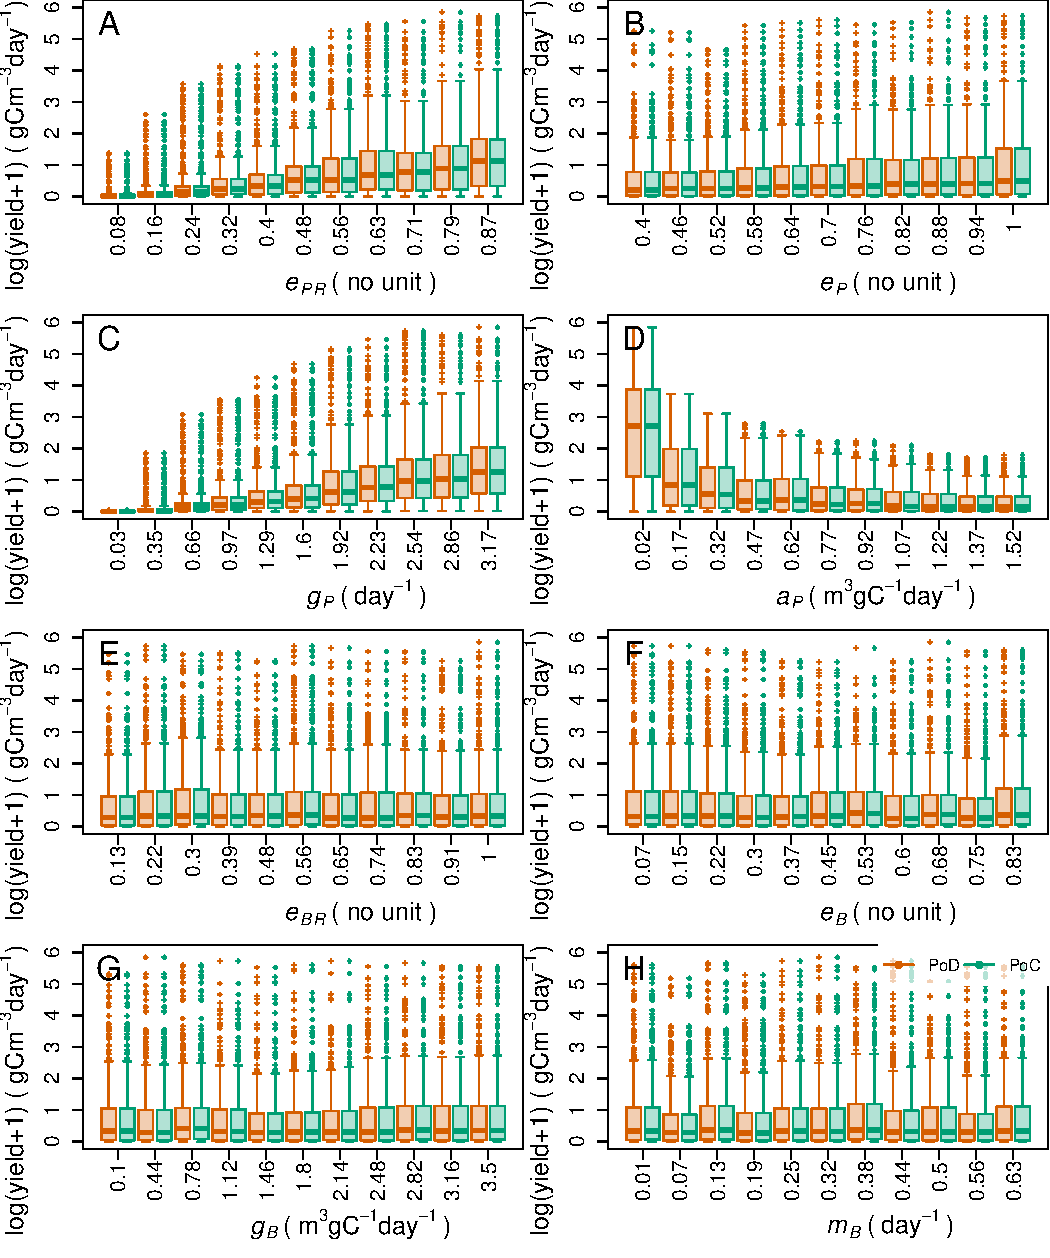
\includegraphics[width=.95\linewidth]{result/harvP.pdf}
    \caption[Log yield flux comparisons between \phy-only systems]{Log yield flux comparisons between \phy-only systems along respective parameter ranges under a standardised temperature range of \temp.  For each independent variable value, the box on its left represented \PoN\ while the one on the right represented \PoH.  Full description of variables were in Table \ref{t:ranges}.  Each group in each plot had an LHS sample size of 5500.  Pairwise Wilcox test showed significance (p $\ll$ 0.01) between the systems.  Note that actual plotted values were not having apparent difference, indicating that the statistical significance may not also have biological significance.}
    \label{f:harvPo}
\end{figure}

\end{document}
